\documentclass[epsf,epic,eepic,eepicemu]{article}\oddsidemargin=-5mm
\evensidemargin=-5mm\marginparwidth=.08in \marginparsep=.01in
\marginparpush=5pt\topmargin=-15mm\headheight=12pt
\textwidth=15cm\columnsep=2mm
\columnseprule=1pt\parindent=15pt\parskip=4pt

\usepackage[T1]{fontenc}
\usepackage[czech]{babel} % recommended if you write in Czech

\usepackage{xcolor}
\definecolor{codeblue}{rgb}{0.2,0.2,1}
\definecolor{codered}{rgb}{1,0.2,0.2}
\definecolor{codegreen}{rgb}{0.2,0.6,0.2}
\definecolor{codemagenta}{rgb}{0.6,0.2,0.6}

\usepackage{float}

\usepackage{listings}
\lstset{
    basicstyle=\ttfamily\small,
    language=C,
    tabsize=2,
    showstringspaces=false,
    breaklines=true,
    captionpos=b,
    keywordstyle=\color{codeblue}\ttfamily,
    stringstyle=\color{codered}\ttfamily,
    commentstyle=\color{codegreen}\ttfamily,
    morecomment=[l][\color{codemagenta}]{\#}
}

\usepackage{caption}
\renewcommand{\lstlistingname}{Kód}% Listing -> Kód

\usepackage{graphicx}
\usepackage{url}

\begin{document}
\begin{center}
\bf Semestrální projekt NI-PDP 2022/2023\\[5mm]
    Paralelní algoritmus pro hledání\\minimálního hranového řezu hranově ohodnoceného grafu\\[5mm] 
       Bc. Luboš Zápotočný\\[5mm]
FIT ČVUT\\Thákurova 9, 160 00 Praha 6\\[2mm]
\today
\end{center}

\section{Definice pojmů a popis sekvenčního algoritmu}

V této kapitole se budeme věnovat definici problému a popisu sekvenčního algoritmu pro řešení minimálního hranového řezu v hranově ohodnoceném grafu. Nejprve připomeneme základní pojmy týkající se grafů a hranového řezu a poté představíme konkrétní problém, který se v této práci řešil.

Problém minimálního hranového řezu v hranově ohodnoceném grafu spočívá v nalezení dvou disjunktních podmnožin uzlů, takzvaných X a Y, takových, že součet ohodnocení všech hran spojujících uzly z obou množin je minimální. Tento problém má mnoho praktických aplikací, například v oblasti sítí, kde se hledají nejlevnější cesty mezi uzly sítě.

Vstupní data obsahují číslo reprezentující počet vrcholů v grafu a následně reprezentaci ohodnocení hran pomocí matice sousednosti. Ukázka vstupních dat je vyobrazena v ukázce \ref{lst:inputExample}.

\begin{lstlisting}[label=lst:inputExample, caption={Vstupní data},language={}]
10
     0   112     0     0    98    80     0     0    91   102
   112     0    90     0     0     0     0   119    96     0
     0    90     0     0   104   111    82     0     0   107
     0     0     0     0     0   114    96     0     0     0
    98     0   104     0     0   118    80    88     0     0
    80     0   111   114   118     0   105   106     0   105
     0     0    82    96    80   105     0   109    93    99
     0   119     0     0    88   106   109     0     0    83
    91    96     0     0     0     0    93     0     0    95
   102     0   107     0     0   105    99    83    95     0
\end{lstlisting}

Sekvenční algoritmus pro řešení tohoto problému je založen na postupném procházení některých (nikoli všech) kombinací podmnožin uzlů X a Y a hledání takové kombinace, která minimalizuje součet ohodnocení hran mezi nimi. 

Některé kombinace algoritmus vynechává, jelikož nemůžou vést k lepšímu řešení, než je aktuálně nalezené minimum. Při průchodu stromem možných kombinací některé podstromy můžeme vynechat. Této metodě se říká Branch and Bound.

Princip prořezávání pomocí Branch and Bound spočívá v systematickém prohledávání stromu kombinací s cílem najít optimální řešení s co nejmenším počtem vyhodnocených kombinací. Algoritmus začíná v kořeni stromu a postupně prochází všechny jeho větve, přičemž se snaží minimalizovat horní hranici ceny řešení a zároveň maximalizovat dolní hranici ceny řešení. Toho se dosahuje pomocí prořezávání podstromů, které nemohou obsahovat optimální řešení.

Prořezávání probíhá pomocí dvou technik: dolních a horních odhadů. Dolní odhady se používají k identifikaci podstromů, které neobsahují optimální řešení, a mohou být tedy bezpečně prořezány. Horní odhady se používají k minimalizaci počtu vyhodnocených kombinací tím, že prořezávají podstromy, jejichž řešení by bylo horší než nejlepší nalezené řešení. Ukázka kódu \ref{lst:cutUpperBound} zobrazuje implementaci horního řezu. Ukázka kódu \ref{lst:cutLowerBound} znázorněna podmínka pro řez pomocí dolního odhadu.

\begin{lstlisting}[float,label=lst:cutUpperBound, caption={Horní řez}]
if (currentWeight >= bestWeight) {
    upperBoundCounter++;
    return;
}
\end{lstlisting}

\begin{lstlisting}[float,label=lst:cutLowerBound, caption={Dolní řez}]
int lowerBound = graph.cutLowerBound(cut, index);

if (currentWeight + lowerBound >= bestWeight) {
    lowerBoundCounter++;
    return;
}
\end{lstlisting}

Dolní odhad je spočítán tak, že pro každý zatím nepřiřazený uzel grafu v daném mezistavu s částečným řezem vypočteme, o kolik by se váha řezu zvýšila, pokud by tento uzel patřil do X, o kolik by se zvýšila, pokud by tento uzel patřil do Y a vezmeme menší z těchto dvou hodnot a tato minima posčítáme pro všechny nepřiřazené uzly.

Cílem prořezávání stromu kombinací pomocí Branch and Bound je minimalizovat počet vyhodnocených kombinací a najít optimální řešení. Tento algoritmus je velmi účinný pro řešení problémů, kde je prostor kombinací velký a výpočetní čas je omezený. \cite{coursesPDPBFS}

Rekurzivní části algoritmu jsou vyobrazeny na ukázkách \ref{lst:recursiveDef} a \ref{lst:recursiveCall}.

\begin{lstlisting}[float,label=lst:recursiveDef, caption={Prototyp rekurzivní funkce}]
void DFS_BB(const Graph &graph, int maxPartitionSize,
            bool *cut, int count, int index,
            int currentWeight, int &bestWeight);
\end{lstlisting}

\begin{lstlisting}[float,label=lst:recursiveCall, caption={Rekurzivní volání}]
// try with this vertex
cut[index] = true;

// try with this vertex (need to extend current cut)
DFS_BB(graph, maxPartitionSize,
       cut, count + 1, index + 1,
       currentWeight + graph.vertexWeight(cut, index, index), bestWeight);

// restore the status of the cut
cut[index] = false;

// try without this vertex (need to extend current cut)
DFS_BB(graph, maxPartitionSize,
       cut, count, index + 1,
       currentWeight + graph.vertexWeight(cut, index, index), bestWeight);
\end{lstlisting}

Za předpokladu, že je nalezeno lepší řešení, je tato hodnota uložena a rekurzivní prohledávání této cesty ve stromu kombinací je u konce. Kód \ref{lst:recursiveBest} zobrazuje část rekurzivní funkce, která kontroluje aktuální váhu řezu a aktualizuje globální proměnnou v případě nalezení lepšího řešení.

\begin{lstlisting}[float,label=lst:recursiveBest, caption={Prototyp rekurzivní funkce}]
if (index == graph.size) {
    if (count != maxPartitionSize) {
        return;
    }

    if (currentWeight < bestWeight) {
        bestWeight = currentWeight;
    }
    
    return;
}
\end{lstlisting}

\section{Popis paralelního algoritmu a implementace v OpenMP - taskový paralelismus}

Taskový paralelismus se používá v OpenMP pro paralelizaci běhu algoritmu. Jednotlivé úlohy (nebo podúkoly) jsou přiděleny vláknům k vykonání. V OpenMP lze k vyznačení úloh použít direktivu \uv{\#pragma omp task}, která říká, že se má daná část kódu vykonat jako samostatná úloha. Ukázka této modifikace je zobrazena v kódu \ref{lst:task}. Přidáním těchto direktiv povolujeme spuštění podúkolů paralelně. Je však důležité, aby tuto rekurzivní funkci započalo pouze jedno vlákno. Proto byla vytvořena separátní funkce, jejíž obsah je zobrazen v ukázce kódu \ref{lst:taskStart}.

\begin{lstlisting}[float,label=lst:task, caption={Modifikace na taskový paralelismus v rekurzivní funkci}]
// try with this vertex (need to extend current cut)
#pragma omp task default(none) firstprivate(graph, cut, count, index, currentWeight)
{
    // try with this vertex
    cut[index] = true;

    // compute weight with this vertex
    int nextWeight = currentWeight+graph->vertexWeight(cut, index, index);

    DFS_BB(cut, count + 1, index + 1, nextWeight);
}

// try without this vertex (need to extend current cut)
#pragma omp task default(none) firstprivate(graph, cut, count, index, currentWeight)
{
    // restore the status of the cut
    cut[index] = false;

    // compute weight without this vertex
    int nextWeight = currentWeight+graph->vertexWeight(cut, index, index);

    DFS_BB(cut, count, index + 1, nextWeight);
}
\end{lstlisting}

\begin{lstlisting}[float,label=lst:taskStart, caption={Začátek taskového paralelismu}]
bestWeight = std::numeric_limits<int>::max();

#pragma omp parallel default(none) firstprivate(graph)
{
    #pragma omp single
    DFS_BB(Cut(graph->size), 0, 0, 0);
}

return bestWeight;
\end{lstlisting}

Více podúkolů může být spuštěno současně a vlákna, která jsou k dispozici, mohou vykonávat úlohy paralelně. Každé dvě podúlohy nezávislé a mohou běžet současně bez čekání na dokončení jiných úloh.

Taskový paralelismus je vhodný pro aplikace s dynamickým vytvářením úloh, které mohou být vykonány asynchronně. To může zvýšit využití výpočetních zdrojů a zlepšit výkon aplikace.

\section{Popis paralelního algoritmu a implementace v OpenMP - datový paralelismus}

Datový paralelismus je druh paralelizace, který spočívá v rozdělení dat na části a zpracování těchto částí v paralelních výpočetních jednotkách.

V programu jednotlivá vlákna zpracovávají různé části dat a zpracování probíhá paralelně. Vhodnou implementací datového paralelismu lze výrazně zlepšit výkon programu, zvláště u algoritmů, které pracují s velkými objemy dat.

Datový paralelismu začíná vygenerováním několik počátečních stavů, které se následně v paralelní smyčce nechávají sekvenčně dopočítat.

Sekvenční algoritmus a taskový paralelismus využívání DFS průchod stromem kombinací. Datový paralelismus nejprve provede BFS expanzi z počátečního vrcholu do dané hloubky a tyto stavy poté nechává více vláknově dopočítat. Ukázka této expanze je v kódu \ref{lst:BFSExpansion}. Tento kód projde stromem kombinací až do hloubky $(2 * maxPartitionSize) / 3$, což je experimentálně zvolená hodnota, která vygeneruje dostatečný počet počátečních stavů. Na konci je výsledné pole počáteční stavů setříděné podle částečné aktuální váhy, což zrychluje nalezení menších hodnot, což poté využívá Branch and Bound pro horní řez některých podstromů výpočtu.

\begin{lstlisting}[float,label=lst:BFSExpansion, caption={BFS expanze před zahájením datového paralelismu}]
auto initialStates = std::vector<State>();
    auto initialStatesQ = std::queue<State>();

    initialStatesQ.push(State(0, 0, 0, Cut(graph->size)));

    while (!initialStatesQ.empty() && initialStatesQ.front().index < (2 * maxPartitionSize) / 3) {
        auto state = initialStatesQ.front();
        initialStatesQ.pop();

        auto cut = Cut(state.cut);

        int nextWeight = state.currentWeight + graph->vertexWeight(cut, state.index, state.index);
        initialStatesQ.push(State(state.count, state.index + 1, nextWeight, cut));

        if (state.count + 1 > maxPartitionSize) continue;

        cut = Cut(state.cut);
        cut[state.index] = true;

        nextWeight = state.currentWeight + graph->vertexWeight(cut, state.index, state.index);
        initialStatesQ.push(State(state.count + 1, state.index + 1, nextWeight, cut));
    }

    while (!initialStatesQ.empty()) {
        initialStates.push_back(initialStatesQ.front());
        initialStatesQ.pop();
    }

    std::sort(initialStates.begin(), initialStates.end());
\end{lstlisting}


\section{Popis paralelniho algoritmu a jeho implementace v MPI}

MPI (Message Passing Interface) je knihovna umožňující programátorům psát paralelní aplikace pro distribuované systémy, které mohou běžet na mnoha procesorech. MPI aplikace jsou psány jako soubor nezávislých procesů, které se navzájem komunikují pomocí posílání zpráv.

MPI umožňuje programátorům psát různé typy paralelních aplikací, včetně datově paralelních a taskově paralelních aplikací. Datově paralelní aplikace pracují s velkými datovými sadami, které jsou rozděleny mezi různé procesory. Každý procesor pracuje s určitou částí dat a výsledky jsou posléze kombinovány. Úlohově paralelní aplikace jsou aplikace, které se skládají z mnoha úloh, které mohou být spuštěny na různých procesorech a mezi sebou komunikují pomocí posílání zpráv.

MPI umožňuje programátorům psát paralelní aplikace, které mohou běžet na různých typech hardware, včetně lokálních počítačů, clusterů a superpočítačů. MPI poskytuje také mnoho funkcí pro synchronizaci a komunikaci mezi procesy, což umožňuje programátorům psát robustní paralelní aplikace.

MPI aplikace se obvykle skládají z řídícího procesu, který koordinuje běh aplikace a koordinuje komunikaci mezi procesy, a mnoha pracovních procesů, které provádějí výpočetní práci. MPI aplikace mohou být napsány v mnoha jazycích, včetně C, C++ a Fortranu. \cite{mpiwiki}

Úprava z datového paralelismu byla komplikovanější než z taskového na datový paralelismus. Program je rozdělen na dva módy. Proces s $ID = 0$ se stává hlavním procesem a rozesílá mezistavy k dořešení na ostatní procesy, které mohou být i na úplně jiném serveru. MPI varaibta algoritmu stále používá datový paralelismus na úrovni vláken.

Komunikace probíhá pomocí zpráv, které znázorňuje kód \ref{lst:mpitags}. Ukázka kódu \ref{lst:mpisendjob} demonstruje čekání hlavního procesu na volný pracovní stroj. Pokud je některý stroj volný, odešle zprávu a hlavní proces mu následně pošle mezistav na dopočítání. Odesílání probíhá ve dvou zprávách. První zpráva obsahuje metadata o aktuálním stavu společně s poslední aktualizovanou hodnotu nejlepší nalezené váhy z ostatních procesů. Následující druhá zpráva obsahuje booleanské pole reprezentující aktuální rozdělení vrcholů do množin X a Y.

\begin{lstlisting}[float,label=lst:mpitags, caption={MPI tagy a specifické tasky}]
enum MPITag {
    SLAVE_INITIALIZED,
    SLAVE_INITIALIZE_GRAPH_SIZE,
    SLAVE_INITIALIZE_GRAPH,
    SLAVE_TASK,
    SLAVE_JOB_STATE,
    SLAVE_JOB_CUT,
    SLAVE_AVAILABLE,
    SLAVE_RESULT
};

enum MPITask {
    JOB,
    SYNC,
    TERMINATE
};
\end{lstlisting}

\begin{lstlisting}[float,label=lst:mpisendjob, caption={MPI tagy a specifické tasky}]
int slave;
MPI_Recv(&slave, 1, MPI_INT, MPI_ANY_SOURCE, MPITag::SLAVE_AVAILABLE, MPI_COMM_WORLD, MPI_STATUS_IGNORE);

int task = MPITask::JOB;
MPI_Send(&task, 1, MPI_INT, slave, MPITag::SLAVE_TASK, MPI_COMM_WORLD);

int stateBuffer[4] = {bestWeight, state.count, state.index, state.currentWeight};
MPI_Send(stateBuffer, 4, MPI_INT, slave, MPITag::SLAVE_JOB_STATE, MPI_COMM_WORLD);

MPI_Send(state.cut.data, graph->size, MPI_C_BOOL, slave, MPITag::SLAVE_JOB_CUT, MPI_COMM_WORLD);
\end{lstlisting}

Každých sto počátečních mezistavů se všechny pracovní stroje sesynchornizují, aby měli nejaktuálnější nejlepší váhu a jejich interní Branch and Bound řezy byly efektivní.


\section{Naměřené výsledky a vyhodnocení}

Na obrázcích \ref{fig:runtime_15__30_20}, \ref{fig:runtime_15__40_8} a \ref{fig:runtime_20__40_8} jsou vyobrazeny časy běhů jednotlivých variant algoritmu. MPI variantz jsou pojmenované podle toho, kolik procesů měli k dispozici = na kolika oddělených strojích mohli pracovat.
Například mpi\_4 znamená, že program byl spuštěn na jednom stroji, který pracoval jako hlavní proces a na třech strojích, pracujících pouze na výpočtu přidělených podúkolů.

\begin{figure}
\centering
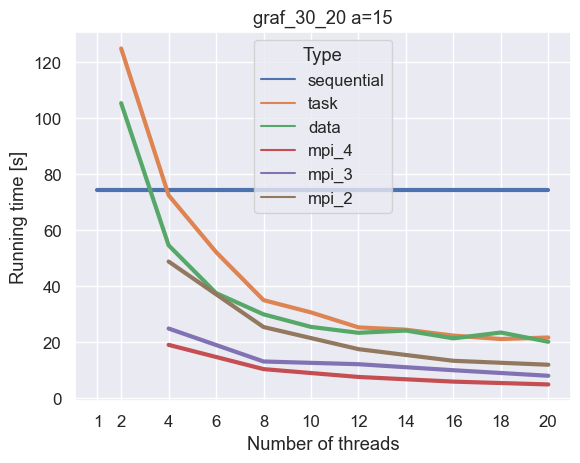
\includegraphics[width=0.75\textwidth]{images/runtime_15__30_20}
\caption{Čas běhu s parametrem 15 na grafu 30\_20}
\label{fig:runtime_15__30_20}
\end{figure}
\begin{figure}
\centering
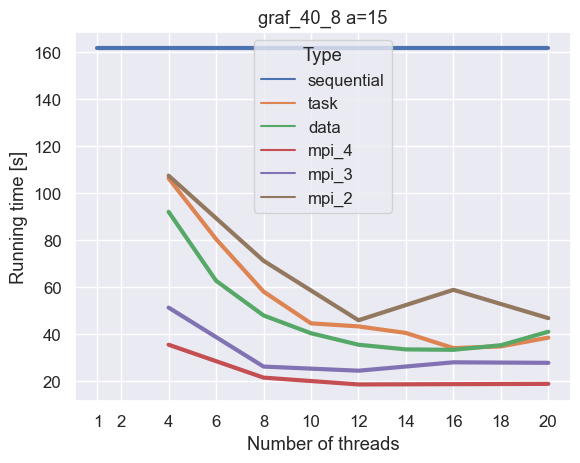
\includegraphics[width=0.75\textwidth]{images/runtime_15__40_8}
\caption{Čas běhu s parametrem 15 na grafu 40\_8}
\label{fig:runtime_15__40_8}
\end{figure}
\begin{figure}
\centering
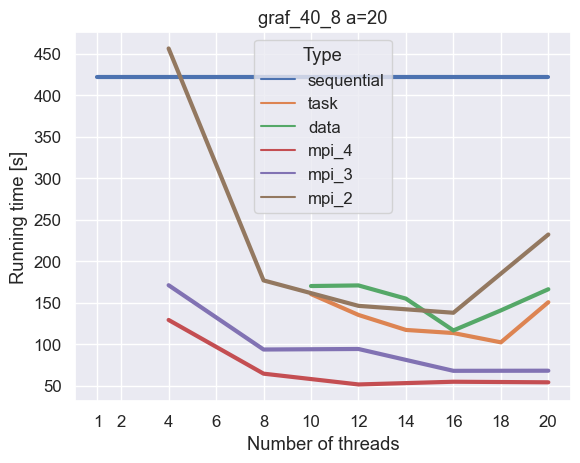
\includegraphics[width=0.75\textwidth]{images/runtime_20__40_8}
\caption{Čas běhu s parametrem 20 na grafu 40\_8}
\label{fig:runtime_20__40_8}
\end{figure}

\begin{figure}
\centering
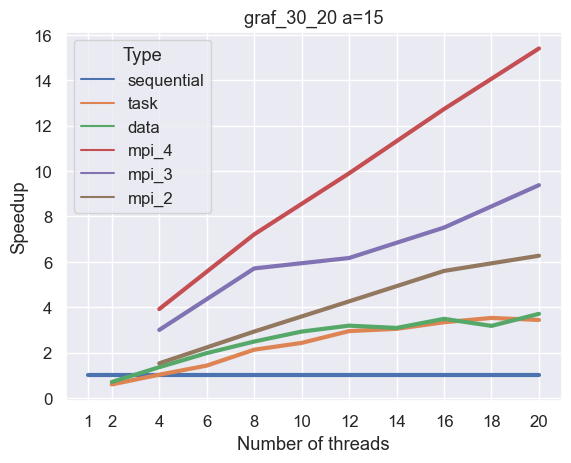
\includegraphics[width=0.75\textwidth]{images/speedup_15__30_20}
\caption{Zrychlení oproti sekvenčnímu řešení s parametrem 15 na grafu 30\_20}
\label{fig:speedup_15__30_20}
\end{figure}
\begin{figure}
\centering
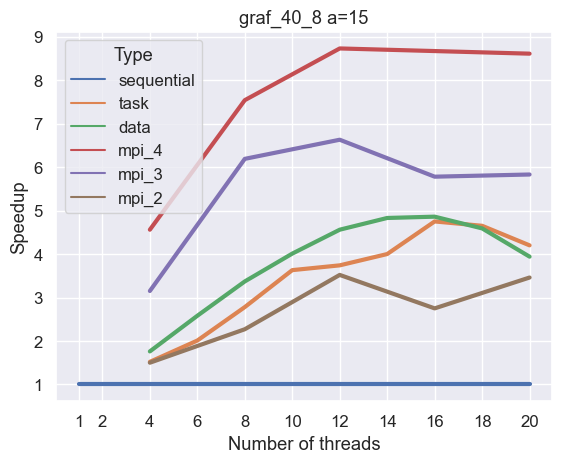
\includegraphics[width=0.75\textwidth]{images/speedup_15__40_8}
\caption{Zrychlení oproti sekvenčnímu řešení s parametrem 15 na grafu 40\_8}
\label{fig:speedup_15__40_8}
\end{figure}
\begin{figure}
\centering
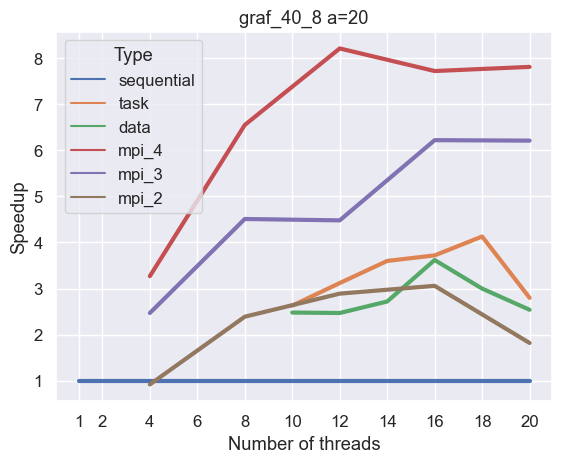
\includegraphics[width=0.75\textwidth]{images/speedup_20__40_8}
\caption{Zrychlení oproti sekvenčnímu řešení s parametrem 20 na grafu 40\_8}
\label{fig:speedup_20__40_8}
\end{figure}

Obrázky \ref{fig:efficency_15__30_20}, \ref{fig:efficency_15__40_8} a \ref{fig:efficency_20__40_8} zobrazují efektivitu paralelního zrychlení, které znázorňuje efektivitu zrychlení podle maximálního počtu vláken k dispozici. U MPI úloh je počet vláken násoben počtem výpočetních uzlů.

\begin{figure}
\centering
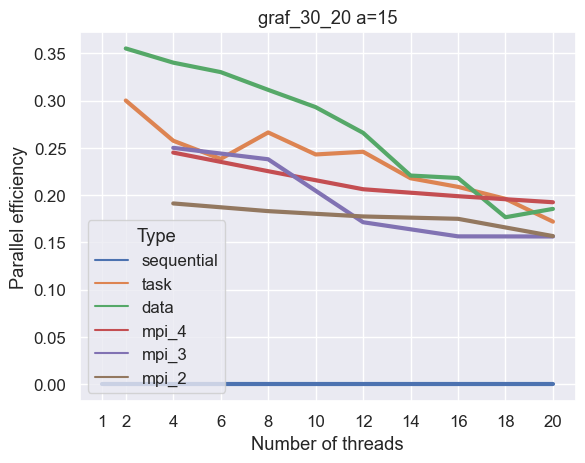
\includegraphics[width=0.75\textwidth]{images/efficency_15__30_20}
\caption{Paralelní efektivita pro vstup s parametrem 15 na grafu 30\_20}
\label{fig:efficency_15__30_20}
\end{figure}
\begin{figure}
\centering
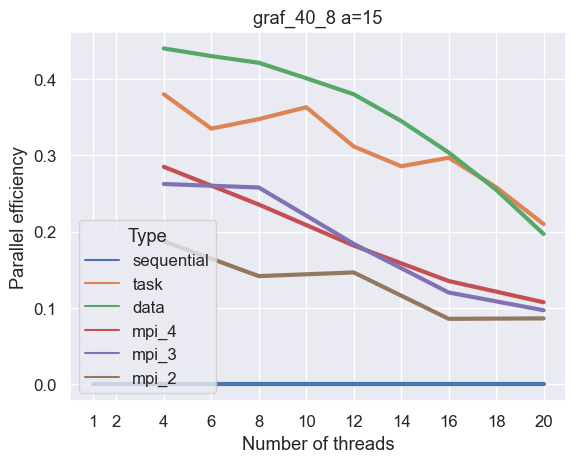
\includegraphics[width=0.75\textwidth]{images/efficency_15__40_8}
\caption{Paralelní efektivita pro vstup s parametrem 15 na grafu 40\_8}
\label{fig:efficency_15__40_8}
\end{figure}
\begin{figure}
\centering
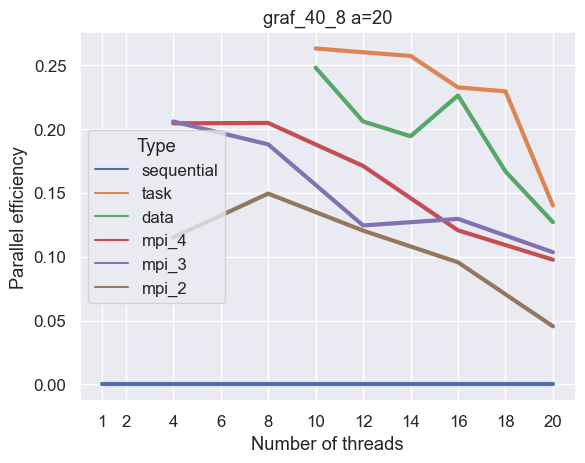
\includegraphics[width=0.75\textwidth]{images/efficency_20__40_8}
\caption{Paralelní efektivita pro vstup s parametrem 20 na grafu 40\_8}
\label{fig:efficency_20__40_8}
\end{figure}

\section{Závěr}

Iterativní práce a postupné modifikace sekvenčního řešení mi dávalo po dobu semestr dobrý smysl a je to takto koncepčně dobře připravené. Doplňkové materiály ke cvičením jsou výborný zdroj pro inspiraci, jakým postupem danou problematiku řešit.

Při použití C++ se mi v některých částech zjednodušila práce s programem (například použitím copy konstruktorů).

Zároveň byla přínosná zkušenost s porovnáním běhu algoritmů na lokálním stroji oproti serverovému clusteru star.

Zde bych chtěl ještě moji práci detailněji prozkoumat, jelikož výsledky prezentované v této zprávě pocházejí ze staru. Na lokálním počítači programy běžely vždy téměř lineárně, což se na startu ani v případě taskového či datového paralelismu nepotvrdilo.

\section{Literatura}

\bibliographystyle{unsrt}
\bibliography{report}

\end{document}
